\chapter{Spatial Modeling}
\label{chap:spatial-modeling}

Spatial modeling of cell electrophysiology first started with neuron via cable
equations.  Early modeling studies first targeted the passive properties, of one
or many interconnected compartments
(Sect.\ref{sec:electrotonus_linearbehavior}).

\section{Principles of spatial modeling}
\label{chap:princ-spat-model}


The most of models we introduced in the previous chapters are based on the basic
assumption of well-mixed (uniform) distribution of chemical concentration inside
each compartment of the cells. There are many situations that this assumption
violates when the size of the cell is big, e.g. the propagation of AP in nerve
cell in which when the cell ``fires'', a wave of membrane depolarization is
initiated at the base of the axon, where it connects to the soma, and propagate
along the axon to its terminus. During the propagation, large spatial gradients
in membrane potentials and local currents are created.

In \ce{Ca^2+} dynamics, the non-uniformity \ce{Ca^2+} concentration at
the vicinity of L-type \ce{Ca^2+} channels was simplicity modeled as a
domain \ce{Ca^2+} in the dyadic subspace. 

A spatial model is a mathematical system that accounts for processes such as
reactions kinetics, diffusion, advection and membrane transport.
\begin{equation}
\begin{split}
\frac{\partial C_i}{\partial t} = -\text{div}F_i + R_i \left( C_j, C_k,
\ldots, \Phi \right)\\
\vec{F_i} = - D_i \nabla C_i - C_i \vec{v_i} - z_i \mu_i C_i \nabla	Phi
\end{split}
\end{equation}
\begin{itemize}
  \item the first equation describes the change in concentration $C_i$ of a
  given species $i$ at a given compartment as a function of time. 
  
This comprised of 2 components: the $R_i$ (reaction part: formation and
degradation of $C_i$; which is a function of any of the other molecular species
in the system, as well as the electrical potential across the membrane, $\Phi$,
if the species is the ion channel and is voltage-sensitive membrane bound
species); (2) the divergence of the flux of species $i$, $F_i$.

  \item Ci can also vary over spatial coordinates, x,y,z; as described via the 
  the Nernst-Planck flux equation $F_i$ with an added advection term
  \begin{enumerate}
    \item  the gradient of concentration times the diffusion coefficient, $D_i$
  
    \item the velocity field $\vec{v_i}$ (possibly driven by molecular
motors)

    \item an electrical term driven by $\nabla \Phi$ is the voltage gradient;
    with  $z_i$ is the charge, $\mu_i$ is the electrical mobility.

NOTE: the electrical term is unimportant within the cytosol, but can, of course,
control ionic transport across membranes.

  \end{enumerate}

NOTE: You equation can ignore one or many of these terms, if needed.  
  
\end{itemize}

The basic tool in modeling the temporospatial dynamic of a substance
is the {\it reaction-diffusion} equations. It is the consequence of
{\it conservation law} which states that some quantity is created or
destroyed within the space defined or moves about (to other space). 

The system is divided into a number of small compartments, in which
the concentration is assumed to be uniform in a compartment R, but not
inter-compartment. So, the time rate of change of the total amount of
C within R is equal to
\begin{verbatim}
  rate at which C flows into R
- rate at which C flows out of R
+ rate at which C is produced within R
- rate at which C is destroyed within R
\end{verbatim}

\subsection{1D formulation (axial diffusion)}
\label{sec:1d-formulation}
\label{sec:axial-diffusion}

The concentration of the species C at the location $x$, at time $t$, is
$c(x,t)$, as shown in Fig.~\ref{fig:diffusion_1D}. Then, within the small slice
of tube between $x$ and $x+dx$, the total concentration of C is $c(x,t)Adx$ with
$A$ is the cross-section area.
The unit of $c(x,t)$ is {\bf amount/volume}, e.g. molar (= mole/litre) or
molecules per unit volume, then the total amount of C is in moles.

\begin{figure}[hbt]
 \centerline{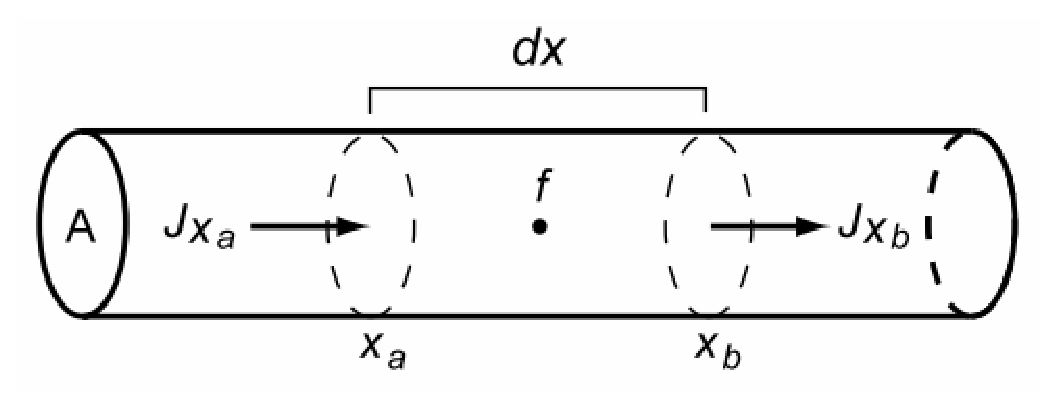
\includegraphics[height=4cm, angle=0]{./images/1D_diffusion.eps}}
\caption{Diffusion in 1D}
\label{fig:diffusion_1D}
\end{figure}

\begin{mdframed}
The total concentration is some arbitrary interval $x_a<x<x_b$ is
\begin{equation}
  \label{eq:797}
  \int_{x_a}^{x_b} c(x,t)Adx
\end{equation}
\end{mdframed}

% Here, we denotes $J_{x_a}, J_{x_b}$ as the flux at which C moves across the
% boundaries, i.e. into and out of the compartment of length $dx$, respectively.
Here, we denotes $J_{x_a}, J_{x_b}$ as the flux at which C moves across the
boundaries, i.e. into and out of the compartment of length $dx$, respectively.
Then, the next movement or {\bf flux}
\begin{equation}
  \label{eq:798}
 \text{net rate of entry} =  AJ_{x_a} - AJ_{x_b} = A (J_{x_a}-J_{x_a+dx})
\end{equation}
which can increase or decrease the concentration an amount
$A dx \frac{\partial c(x,t)}{\partial t}$.

Divided both sides by $Adx$
\begin{equation}
\frac{J_{x_a} - J_{x_a+dx}}{dx} = A (J_{x_a}-J_{x_a+dx}) = \frac{\partial
c(x,t)}{\partial t}
\end{equation}
In the limit of $dx \rightarrow 0$ (and $x_a < x_a+dx$), then
\begin{equation}
-A\frac{\partial J}{\partial x} = \frac{\partial
c(x,t)}{\partial t}
\end{equation}
To help finding the left-hand side, we use Fick's law
(Sect.\ref{sec:ficks-law-diffusion}) as given in eq.\ref{eq:Fick-law}.
The final formula is
\begin{equation}
D \times A \frac{\partial^2}{\partial x^2} c(x,t)= \frac{\partial
c(x,t)}{\partial t}
\end{equation}
with $D$ (diffusion constant), $A$ (cross-seciontional area).
 
\begin{framed}
The unit of net rate of entry is amount/time. Thus, the unit of $J$ is
{\bf amount/area/time}.

Important notation: $J(x,t)$ is positive when C moves to the right,
and $J(x,t)$ is negative when C moves to the left. 
\end{framed}

\subsection{Fick's law of diffusion}
\label{sec:ficks-law-diffusion}

Fick's law of diffusion states that a species C moves from a place of
higher concentration to place of lower concentration; and the rate of
movement $J$ is proportional to the concentration gradient.

Fick's first law:
\begin{eqnarray}
  \label{eq:406}
  J_{diff} = -D \frac{\partial}{\partial x} c(x,t)
\end{eqnarray}
with $D$ is the diffusion constant whose value depends on the size of
C, as well as the properties of the medium. The unit of $D$ is
{\bf length$^2$/time}. The negative sign means C moves spontaneously
from region of high concentration to regions of low concentration. 

So
\begin{equation}
\label{eq:Fick-law}
\frac{\partial J}{\partial x} = -D \frac{\partial^2}{\partial
x^2} c(x,t)
\end{equation}

% In a general case, where the cross-sectional area is not unit, but of $A$
% (cm$^2$), then
% \begin{equation}
% \label{eq:Fick-law}
% \frac{\partial J}{\partial x} = -D \times A \frac{\partial^2}{\partial x^2}
% c(x,t)
% \end{equation}


For example:
\begin{itemize}
\item D: cm$^2$/sec
\item $[c(x,t)]$: moles/cm$^3$.
\item $J_{diff}$: moles/(sec.cm$^2$).
\end{itemize}

\subsection{2D formulation (axial diffusion + radial diffusion)}

In a dendrite, which is roughly cylindrical, diffusion may be radial - flowing
from spines and calcium channels toward the center of the dendrite
\citep{DeSchutter1998}.  Thus, a more accurate representation should include 2D
diffusion.

STRATEGY: Subdivision of three dimensional cylinder into rings for axial and
radial diffusion.

\begin{equation}
\frac{\partial c(x,t)}{\partial t} =
D \left( \frac{\partial^2}{\partial x^2} c(x,t) + 
\frac{1}{r}\frac{\partial }{\partial r}c(x,t) +
\frac{\partial^2}{\partial r^2} c(x,t)
 \right) 
\end{equation}


\subsection{Reaction-Diffusion equation}
\label{sec:react-diff-equat}

Consider $f(x,t,c(x,t))$ as the function that represents the net rate
of increase of C (i.e. production - destruction)
{\it per unit volume at} location $x$ and time $t$, then the total
amount of C produced in the compartment at time $t$ is
\begin{equation}
  \label{eq:799}
 \text{net rate of production} = \int_{x_a}^{x_b} f(x,t,c(x,t)) A dx
\end{equation}
Since the unit of net rate of production is amount/time; the unit of
$f(\cdot)$ is {\bf amount/time/volume}.

\begin{framed}
  When $f(\cdot)$ is negative, C is consumed. $f$ is called the source
  function. 
\end{framed}

So, we formulate the change of C in the compartment
\begin{equation}
  \label{eq:800}
  \frac{d}{dt}\int_{x_a}^{x_b} c(x,t) A dx = A[J(x_a,t)-J(x_b,t) + \int_{x_a}^{x_b} f(x,t,c(x,t)) dx]
\end{equation}
If we write the flux in a general form $J(t)$, then
$J(x,t)=\frac{\partial}{\partial x} J(x,y,z,t)$. 
Finally, all the terms in eq.~\eqref{eq:800} can be written in
integral form
\begin{equation}
  \label{eq:801}
  \frac{d}{dt}\int_{x_a}^{x_b} c(x,t) A dx =
  A[\int_{x_a}^{x_b}\frac{\partial}{\partial x} J(x,y,z,t) dx  + \int_{x_a}^{x_b} f(x,t,c(x,t)) dx]  
\end{equation}

If the function $c(x,t)$ is smooth, then integration and
differentiation can be interchanged 
\begin{equation}
  \label{eq:802}
  \int_{x_a}^{x_b}\left[  \frac{\partial}{\partial t} c(x,t) A  -
  A[\frac{\partial}{\partial x} J(x,y,z,t)   -  f(x,t,c(x,t)) ]\right]
dx = 0
\end{equation}
Since the interval is arbitrary, the only way for this equality to
hold is the integrand to be zero, i.r. 
\begin{equation}
  \label{eq:803}
  \frac{\partial}{\partial t} c(x,t)  =
    \frac{\partial}{\partial x} J(x,y,z,t)   +  f(x,t,c(x,t)) 
\end{equation}
The {\bf law of conservation} only give us one equation, eq.~\eqref{eq:803}
However, with two unknown variable, we need a second one. The second
one is obtained from Ficks' law of diffusion.


Combine eq.~\eqref{eq:803} and eq.~\eqref{eq:406}, we obtain the
so-called {\bf reaction-diffusion} equation
\begin{equation}
  \label{eq:804}
  \frac{\partial}{\partial t} c(x,t) =
  \frac{\partial}{\partial x} \left( -D\frac{\partial}{\partial x}
    c(x,t) \right)   +  f(x,t,c(x,t)) 
\end{equation}
or
\begin{equation}
  \label{eq:805}
  \frac{\partial}{\partial t} c(x,t) = - D\frac{\partial^2}{\partial x^2} 
  \left(c(x,t) \right)   + f(x,t,c(x,t)) 
\end{equation}

\subsection{Advection}
\label{sec:advection}

In the case that the solve also flow, with speed $v_x$ along the
$x-$axis. The movement of C caused by the movement of the solvent is
called {\bf advection}. 
\begin{equation}
  \label{eq:806}
  J_{adv} = vc(x,t)
\end{equation}
Then, the movement of particles of species C is the combination of
both diffusion and advection.
\begin{equation}
  \label{eq:807}
  J = J_{adv} + J_{diff} = vc(x,t) - D\frac{\partial}{\partial t} c(x,t)
\end{equation}


\subsection{Drift (for charged particle)}
\label{sec:drift-for-charged}

Now, we considered a more complicated situation, when the substance C
is an ion. Then, the movement of ions is also driven by the potential
difference; and the movement is now called the current.

The flux of ions is given by the {\bf Nernst-Plank} equation
\begin{equation}
  \label{eq:808}
  J_{driff} = -D \left( \frac{\partial}{\partial t}c(x,t) +
    \frac{zF}{RT}c(x,t) \frac{\partial \phi}{\partial t} \right)
\end{equation}
with $z$ is the valence of the ions (e.g. $z_{\ce{Ca}}=2, z_{\ce{Na}}=1$);
$F$ is the Faraday's constant, $R$ is the universal constant, $T$ is the
temperature (K).

One common example is the movement of ions across the ion channels. 

\section{Numerical method of diffusion}

The discretization leads to the diffusion flux
\def\ion{{\text{ion}}}
\def\Dif{{\text{Diffusion}}}
\begin{equation}
\Phi_\Dif = J_{i\rightarrow j} = - D \frac{A_{ij}}{\Delta s_{ij}} \left(
[\ion]_i - [\ion]_j\right)
\end{equation}
with $A_{ij}$ is the cross-sectional area between two compartments $i$ and $j$;
$\Delta s_{ij}$ is the distance between the two central points of the two
compartments (where $[\ion]_j, [\ion]_j$ are measured).

The change in $[\ion]$ in the compartment $i$, caused by the diffusion flux
$J_{i\rightarrow j}$ will be determined by the volume $v$ in which 
$J_{i \rightarrow j}$ is diluted.
\begin{itemize}
  \item Euler method
  \item Crank-Nicholson method
\end{itemize}

\subsection{Euler method}
\label{sec:Euler-method-ion-diffusion}

The loss is at one end, i.e. from $i$ to $j=(i+1)$
\begin{equation}
[\ion]_{i,t+\Delta t} - [\ion]_{i,t} = \Delta t \times D_\ion \times
\frac{A_{ij}}{\Delta s_{ij}^2 \times v_i} \left(
[\ion]_{i+1,t} - [\ion]_{i,t}\right)
\end{equation}
with $j=i+1$, $v_i$ is volume of compartment $i$.

\begin{equation}
[\ion]_{i,t+\Delta t} - [\ion]_{i,t} = \Delta t \times D_\ion \times
\frac{A_{ij}}{\Delta s_{ij}^2 \times v_i} \left(
[\ion]_{i+1,t} - [\ion]_{i,t}\right)
\end{equation}

The coupling constant (unit: 1/$\mum^2$)
\begin{equation}
C_{i,j} = \frac{A_{ij}}{\Delta s_{ij} \times v_i} 
\end{equation}
depends on the specific geometry of the compartment, and will usually be
different for any pair of compartments.

The loss is at two ends, i.e. from $i$ to both $j=(i+1)$ and $k=(i-1)$.
The central difference is used
\begin{equation}
[\ion]_{i,t+\Delta t} - [\ion]_{i,t} = \Delta t \times D_\ion \times
\frac{A_{ij}}{\Delta s_{ij}^2 \times v_i} \left(
[\ion]_{i+1,t} - 2[\ion]_{i,t} + [\ion]_{i-1,t}\right)
\end{equation}

\subsection{Crank-Nicholson method}
\label{sec:Crank-Nicholson-method-ion-diffusion}

With time step $\Delta t$.

\subsection{Crank-Nicholson-Hines method}
\label{sec:Crank-Nicholson-Hines-method-ion-diffusion}

With time step $\Delta t/2$.

The loss is at one end, i.e. from $i$ to $j=(i+1)$
\begin{equation}
\begin{split}
&[\ion]_{i,t+\Delta t} - [\ion]_{i,t} =\\
& \frac{\Delta t}{2} \times D_\ion
\times \frac{A_{ij}}{\Delta s_{ij} \times v_i} \left(
\left([\ion]_{i+1,t+\Delta t/2} - [\ion]_{i+1,t+\Delta t/2} +
\right)
\left(
[\ion]_{i+1,t} - [\ion]_{i+1,t} 
\right)
\right)
\end{split}
\end{equation}
with $j=i+1$, $v_i$ is volume of compartment $i$.

The loss is at two ends, i.e. from $i$ to both $j=(i+1)$ and $k=(i-1)$,
i.e. both $(i+1)$ and $(i-1)$ compartments are used in
calculating $i$-compartment
\begin{equation}
\begin{split}
&[\ion]_{i,t+\Delta t} - [\ion]_{i,t} =\\
& \frac{\Delta t}{2} \times D_\ion \times
\frac{1}{v_i} 
\left(
A_{i,i+1}
\frac{\left([\ion]_{i+1,t+\Delta t/2} - [\ion]_{i,t+\Delta t/2} 
\right)}{\Delta s_{i,i+1}} -
A_{i,i-1}\frac{\left(
[\ion]_{i,t} - [\ion]_{i-1,t} 
\right)}{\Delta s_{i,i-1} }
\right)
\end{split}
\end{equation}

\subsection{Initial and Boundary conditions}
\label{sec:init-bound-cond}

To solve an ODE, we need some initial conditions. To solve a PDE, we
need both initial conditions (for time), and boundary conditions (for
space). 

\begin{framed}
A problem, i.e. a set of ODEs, is an {\bf initial-value problem}, when we know
the information of all dependent variables (x,y,\ldots) at a single value of
the independent variable (e.g. $t=0$).

A problem, is a {\bf boundary-value problem}, when we know only the condition at
given different values of the independent variable, e.g. $x(t=0)=x_0$ and
x(t=$t_f)=x_f$; but we don't know values of y. In a boundary-value problem, the
values that we know are often given at the  extreme points or boundaries of the
system. That's why we call them that name.

\end{framed}

In many cases, time-variable are initial-value problem; and boundary-value
problem arise more naturally when integrating in space. For the problem of
calcium concentration dynamics, at a single grid point, we have
\begin{equation}
c = f(c) + D_x \nabla c
\end{equation}
with $f(c)$ refers to the ``internal" change of c (inside the grid point where
calcium react with other species); and $D_x$ is the diffusion of calcium along
the x-direction, $\nabla$

For each degree of derivative, we need one condition for each
unknown variables. So, in the reaction-diffusion equation in
eq.~\eqref{eq:805}, we need
\begin{itemize}
\item one initial condition for time $t$
\item two boundary conditions for space $x$ (left and right)
\end{itemize}

There are commonly used boundary conditions
\begin{enumerate}
\item Dirichlet condition: the concentration at the boundary to follow
  some function, e.g. $c(x_a,t)=f(t), c(x_b,t) = g(t)$

\item Neumann boundary condition: the rate of change at the boundary
  to follow some function, e.g.
  $-D\frac{\partial}{\partial x}c(x_a,t)=f(t)$.

\item Robin condition (the combination of the two above): the flux at
  the boundary depends on both time and the current concentration,
  e.g.  $-D\frac{\partial}{\partial x}c(x_a,t)=f(t) - \alpha c(x,t)$.
\end{enumerate}

\subsection{Numerical solutions}
\label{sec:numerical-solutions}

\subsection{Shooting method}
\label{sec:shooting_method}

It converts a boundary-value problem into an equivalent initial-value problem,
by adding one or more new variables. Then, a trial-and-arror approach is used.
This method can work for higher-order and non-linear equation. 

Example: The heated rod with temperature T varies along the rod
\begin{equation}
\frac{d^2T}{dx^2} + h'(T_\infty - T) = 0
\end{equation}
with $T(0)=T_a$, $T(L)=T_b$. Then we define a new variable $z=\frac{dT}{dx}$.
and re-express the problem
\begin{equation}
\frac{dz}{dx} = -h'(T_\infty-T)
\end{equation}
and the initial condition is now $T(0) = T_a, z(0)= ????$. Now, we need to make
a guess for $z(0)$. 

We may need to guess many time, and adjust z(0) guess so that calcculated T(L)
is about $T_b$. 

This fixed boundary condition is known as {\bf Dirichlet condition}.

\subsubsection{Simplest method}
\label{sec:simplest-method}


Example: the diffusion of \ce{Ca^2+} in a sealed dendrite of 40 micron
long, e.g.  $x$ ranges from $x_a=0$ to $x_b=40$ microns. Assume that there is no
production/destruction of calcium, then we have the equation
\begin{equation}
  \label{eq:809}
  \frac{\partial}{\partial t} c(x,t) = - D\frac{\partial^2}{\partial x^2} 
  \left(
    c(x,t) \right)   
\end{equation}
where the initial condition is
\begin{equation}
  \label{eq:810}
  c(x,0) = \left\{
    \begin{array}{lc}
      C_0 & 20 \mu m < x < 30 \mu m \\
      0  & \text{ elsewhere } \\
    \end{array}
    \right.
\end{equation}
and the boundary condition is (sealed dendrite)
\begin{equation}
  \label{eq:811}
  c(x_a,t) = c(x_b,t) = 0
\end{equation}
which is the special case of the Dirichlet condition.


For the spatial problem, the dendrite is divided into $N$ equal
intervals, with $\Delta x=40/N$ is the length of each interval. With
$N$ intervals, we have $N+1$ end-points. For easier manipulation,
let's follow this convention
\begin{enumerate}
\item the index for the end-point is $n$
\item the first end-point start at zero $n=0$, the last end-point is
  $n=N$.
\item the index of the compartment is then taken as the index of its
  right end-point.  
\end{enumerate}

\begin{figure}[hbt]
 \centerline{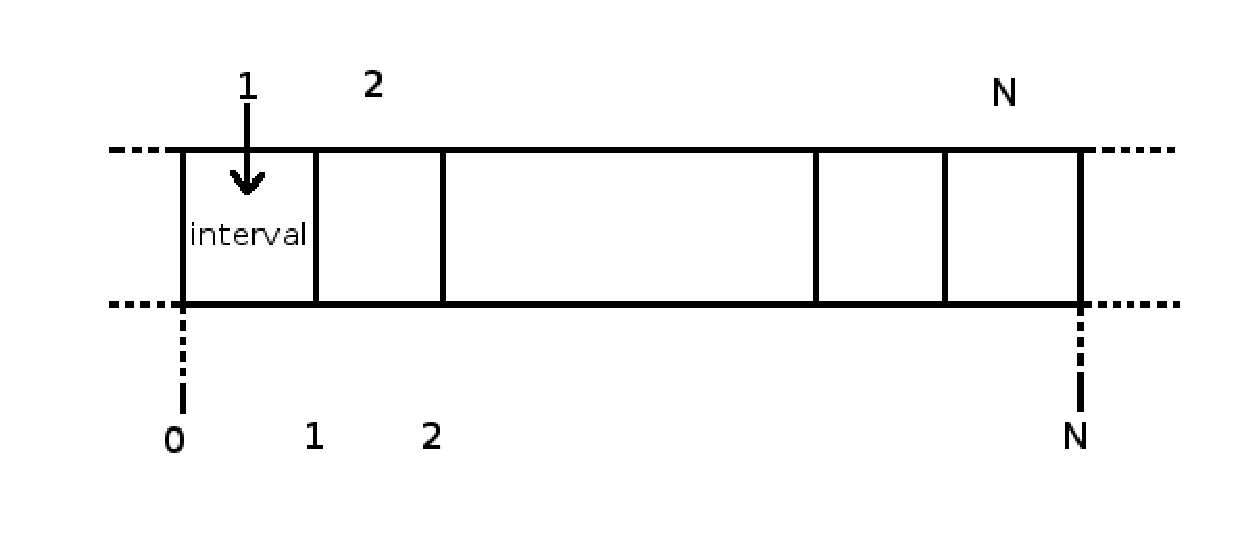
\includegraphics[height=5cm, angle=0]{./images/cell_1D.eps}}
\caption{Schematic diagram of a dendrite divides into intervals in 1D}
\label{fig:cell_1D}
\end{figure}

For the left side of eq.~\eqref{eq:809}, we have an approximation
\begin{equation}
  \label{eq:812}
  \frac{\partial}{\partial t} c(x,t) = \frac{c(x+\Delta x,t) -
    c(x,t)}{\Delta x}
\end{equation}
In a similar way, the approximation for the right side is
\begin{equation}
  \label{eq:813}
  \frac{\partial^2}{\partial x^2} \left(c(x,t) \right)  
  = \frac{c(x+\Delta x,t) - 2c(x,t) + c(x-\Delta
    x,t)}{\Delta x^2}
\end{equation}
using the {\it three-point central difference scheme}. 

Now, we map the continuous $x$ to the discretized index $n$,
$n=1,...,N$
\begin{equation}
  \label{eq:814}
  \frac{\partial }{\partial t} c_n(t) = \frac{D}{\Delta
    x^2}(c_{n+1}(t)-2c_n(t) + c_{n-1}(t))
\end{equation}

How do we know the concentration $c_o(t)$ and $c_{N+1}(t)$.  Now is
the time to apply the boundary conditions
\begin{equation}
  \label{eq:815}
  c_0(t) = 0 \; ; c_{N+1} = 0 
\end{equation}
or the first and last equation can have simpler forms 
\begin{equation}
  \label{eq:816}
  \begin{split}
    \frac{\partial }{\partial t} c_1(t) &= \frac{D}{\Delta
      x^2}(c_{2}(t)-2c_1(t)) \\
    \frac{\partial }{\partial t} c_N(t) &= \frac{D}{\Delta
      x^2}(-2c_N(t) + c_{N-1}(t))    
  \end{split}
\end{equation}

If we invoke the no-flux boundary condition, and substitute it with
the approximation in eq.~\eqref{eq:812}, with the special case of the
Neumann condition $\frac{\partial}{\partial x}c(x,t) = 0$, or
\begin{equation}
  \label{eq:818}
  c_0 = c_1 \; ; c_{N+1} = c_N
\end{equation}
we have
\begin{equation}
  \label{eq:817}
  \begin{split}
    \frac{\partial }{\partial t} c_1(t) &= \frac{D}{\Delta
      x^2}(c_{2}(t)-c_1(t)) \\
    \frac{\partial }{\partial t} c_N(t) &= \frac{D}{\Delta
      x^2}(-c_N(t) + c_{N-1}(t))        
  \end{split}
\end{equation}

Either using eq.~\eqref{eq:816} or eq.~\eqref{eq:817}, combined with
eq.~\eqref{eq:814}, we have a closed system of $N+1$ equations. 
The method of conversion of a PDE to a system of ODE using difference
approximation is called {\bf method of lines}. 

\begin{framed}
  Method of lines (MOL) is a special {\it finite difference method},
  but more effective in terms of accuracy and computational time.  It
  involves discretising a given differential equation in one or two
  dimensions while using analytical solution in the remaining
  direction. It can makes use of state-of-the-art and reliable ODE
  solves. In the above example: the spatial derivatives are
  discretized (approximated using simple finite difference
  relationship), the last direction (the time direction) is solved
  using any chosen ODE solver, e.g. forward Euler method or forward
  stepping Runge-Kutta.
  
  MOL can be used to solve either hyperbolic (wave equation), or
  parabolic or elliptic equation. 

  MOL, however, cannot be used to solve problems with complex
  geometry. 
\end{framed}

